\section{Results}
\label{sec:results}

\paragraph{RQ1: Does the dataset affect quantization robustness?}
Bit width and group size set the level of retention (\cref{fig:bits}): both groups collapse at 1 bit and keep nearly all their accuracy at 8 bits, and they separate in between.
At W3/G128, the UFG group retains \V{retSc_w3g128} against \V{retOther_w3g128} for the FG group, a gap of \V{gap_w3g128}, positive in \V{gapPos_w3} of the \V{nSettingGs} combinations of setting and group size at 3 bits.
Smaller groups move this band to fewer bits (\cref{fig:bits}, right).
\textbf{The dataset effect is therefore a property of the transition band, located by bit width and group size together.}
At 1 bit the gap is negative for BEiTv2 FT, also after chance correction; several of its UFG baselines are near chance, where both measures are unstable.
The gap at W3/G128 survives chance-corrected retention (\V{gapChance_w3g128}), removal of the \V{lowBaseline} baselines below 15\% (\V{gapNoLow_w3g128}), and removal of any one UFG dataset (at least \V{looMinGap}), staying positive in all nine settings (\cref{tab:robust}).
A bootstrap over datasets places its 95\% interval above zero in \V{bootPositive} of the eight settings other than BEiTv2 FT, whose lower bound is \V{bootLowBeitFt}.

Within each setting the four primary conditions agree on the ranking of datasets, with Kendall's $W$ between \V{wMin} and \V{wMax} (\cref{tab:gatesShort}).
Across settings, the median Spearman correlation between two settings' scores is \V{agreeMedian}, ranging from \V{agreeMin} to \V{agreeMax}, and among the FG datasets alone it is only \V{agreeOtherMedian}.
The order between the groups is more stable.
In every setting, a UFG dataset has the higher \term{difficulty score} in at least \V{sepMin} of the pairs of one UFG and one FG dataset, and in all of them in \V{sepOne} of nine settings.
\textbf{The dataset effect is stable at the level of the two groups, while the order within the FG group depends on the backbone and the strategy.}

\begin{table}[t]
\centering
\caption{Agreement $W$ of the four primary conditions on the ranking of the {\V{gridDatasets}} datasets, and Spearman $\rho$ of the difficulty score with the baseline margin $q_{10}$, with baseline top-1, and with $q_{10}$ after controlling for top-1 (partial).}
\label{tab:gatesShort}
\setlength{\tabcolsep}{3pt}
\small
\begin{tabular}{llrrrr}
\toprule
Backbone & Strategy & $W$ $\uparrow$ & $\rho$ ($q_{10}$) & $\rho$ (top-1) & Partial \\
\midrule
ViT-B/16 & FT & 0.89 & $-$0.96 & $-$0.97 & $-$0.28 \\
ViT-B/16 & FZ & 0.93 & $-$0.93 & $-$0.91 & $-$0.51 \\
ViT-B/16 & CAL & 0.81 & $-$0.82 & $-$0.84 & 0.05 \\
Swin-B & FT & 0.81 & $-$0.87 & $-$0.82 & $-$0.54 \\
Swin-B & FZ & 0.95 & $-$0.97 & $-$0.98 & $-$0.45 \\
Swin-B & CAL & 0.73 & $-$0.65 & $-$0.67 & $-$0.05 \\
BEiTv2-B & FT & 0.83 & $-$0.53 & $-$0.45 & $-$0.35 \\
BEiTv2-B & FZ & 0.94 & $-$0.93 & $-$0.96 & 0.21 \\
BEiTv2-B & CAL & 0.91 & $-$0.80 & $-$0.72 & $-$0.56 \\
\bottomrule
\end{tabular}
\end{table}


\begin{figure}[t]
  \centering
  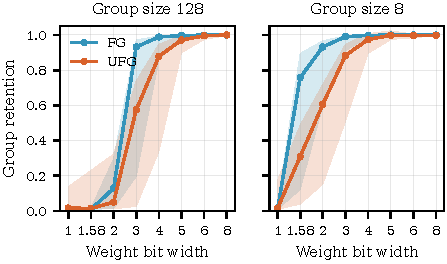
\includegraphics[width=\linewidth]{figures/retention_bits.pdf}
  \caption{Group retention against weight bit width. Lines: median over the nine settings; bands: minimum to maximum. Group means weight the datasets equally.}
  \label{fig:bits}
\end{figure}

\paragraph{RQ2: How and why does the dataset affect it?}
Since prediction changes after quantization concentrate on images with small output margins~\cite{hu2023towards}, we hypothesize that datasets whose baselines have many small-margin images lose more.
The prespecified margin signal holds in all \V{gatePass} settings, with a median $\rho$ of \V{rhoMarginMedian} and $p<0.05$ in all \V{gatePPass} (\cref{tab:gatesShort}).
However, baseline accuracy correlates with the score almost as strongly, with a median $\rho$ of \V{rhoAccMedian}.
Controlling for baseline accuracy, the partial correlation of $q_{10}$ with the score stays negative in \V{partialNeg} of nine settings, with a median of \V{partialMedian} (\cref{tab:gatesShort}): at similar accuracy, datasets with smaller margins are still harder.
Adding $q_{10}$ to the controls, however, lowers the held-out error in only \V{marginHelps} of nine settings.

Baseline accuracy also leaves the retention of individual contexts open (\cref{fig:accuracy} in the appendix).
Of the \V{pairsClose} pairs of datasets within one setting whose baseline top-1 differs by at most 1.5 points, \V{pairsDiffer} differ in retention by more than 0.2, and in \V{differQ10} of these the dataset with the smaller $q_{10}$ retains less.
On BEiTv2 CAL, Cars and Food start from \V{pairALowFp}\% and \V{pairAHighFp}\% but retain \V{pairALowR} and \V{pairAHighR}, and Cars has the smaller $q_{10}$, \V{pairALowQ} against \V{pairAHighQ}.
\textbf{The margin adds rank information beyond baseline accuracy, but not enough to improve a held-out prediction.}


\begin{table}[t]
\centering
\caption{Retention gap (FG $-$ UFG) at W3/G128 before (Raw) and after (Matched) matching the baseline margin distributions, and the reduction of the gap (Red.).}
\label{tab:marginShort}
\setlength{\tabcolsep}{3pt}
\small
\begin{tabular}{llrrr}
\toprule
Backbone & Strategy & Raw & Matched & Red. (\%) \\
\midrule
ViT-B/16 & FT & 0.212 & 0.042 & 80.0 \\
ViT-B/16 & FZ & 0.310 & 0.188 & 39.2 \\
ViT-B/16 & CAL & 0.268 & 0.118 & 55.9 \\
Swin-B & FT & 0.498 & 0.248 & 50.2 \\
Swin-B & FZ & 0.569 & 0.412 & 27.6 \\
Swin-B & CAL & 0.341 & 0.112 & 67.1 \\
BEiTv2-B & FT & 0.408 & 0.188 & 53.9 \\
BEiTv2-B & FZ & 0.184 & 0.078 & 57.4 \\
BEiTv2-B & CAL & 0.325 & 0.061 & 81.3 \\
\bottomrule
\end{tabular}
\end{table}


\begin{figure}[t]
  \centering
  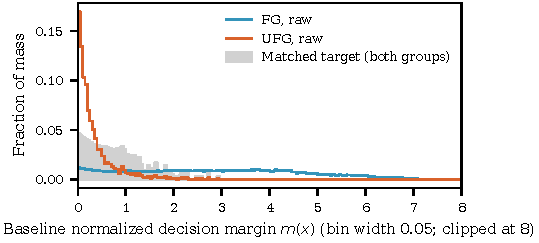
\includegraphics[width=\linewidth]{figures/margin_distribution.pdf}
  \caption{Baseline margin distributions of the two groups for ViT-B/16 FT, before matching, and the common target used for matching. Margins above 8 are not shown.}
  \label{fig:margin}
\end{figure}

Margin matching asks how much of the gap goes with the margins, within the W3/G128 test images, where the UFG images concentrate at small margins (\cref{fig:margin}).
Matching both groups to their common margin distribution reduces the gap by \V{reductionMin}\% to \V{reductionMax}\%, with a median of \V{reductionMedian}\% (\cref{tab:marginShort}).
The matched gap stays positive in \V{matchedPositive} of nine settings, so the UFG images lose more even at equal margin.
The comparison covers only the shared \V{overlapMin} to \V{overlapMax} of the histogram mass, and the matched ESS falls to as little as \V{essRatioMin}\% of the raw ESS (\cref{tab:margin} in the appendix).
Matching aligns only the distance to the second-ranked class, yet a median of \V{beyondSc}\% of the UFG swaps, against \V{beyondOther}\% for the FG datasets, end on a class the baseline ranked below second.
This share follows the margin ($\rho$ \V{beyondRhoMargin} with $q_{10}$) rather than the class count ($\rho$ \V{beyondRhoClasses}).
The top-1 to top-2 margin is therefore a summary of the logits, not a full account of how quantization changes decisions.
\textbf{Much of the retention gap goes with the smaller margins of the UFG images, but not all of it.}

Decisions change far more often for the UFG images.
At W3/G128, a median of \V{w3SwapSc}\% of UFG test images change their prediction, against \V{w3SwapOther}\% of FG images, and the UFG group swaps more in \V{swapHigherSc} of nine settings (\cref{tab:groups}).
Since only \V{w3FpSc}\% of UFG images are correct at baseline, at least \V{wrongSwapScMin}\% of the UFG swaps move between two wrong classes in every setting.

\begin{table}[t]
\centering
\caption{Baseline (FP) and quantized (Q) top-1, and swap, damage and rescue rates at W3/G128, in \%. Each value is the median over the nine settings of the group mean.}
\label{tab:groups}
\setlength{\tabcolsep}{3pt}
\small
\begin{tabular}{lrrrrr}
\toprule
Group & FP & Q & Swap & Damage & Rescue \\
\midrule
UFG & 33.1 & 15.7 & 72.0 & 20.1 & 3.7 \\
FG & 88.1 & 80.7 & 14.4 & 7.5 & 1.6 \\
\bottomrule
\end{tabular}
\end{table}


Feature similarity does not track the loss.
At mid depth, the median CKA between baseline and W3/G128 features is \V{midCkaSc} for the UFG group and \V{midCkaOther} for the FG group.
Final-layer CKA correlates with the score at a median $\rho$ of only \V{rhoCkaMedian} (\cref{tab:properties}).
